\documentclass{article}
\usepackage{latexsym}
\usepackage{amsmath}
\usepackage{amssymb}
\usepackage{epsfig}
\usepackage{caption}
% \usepackage{psfig}
%\usepackage{epic}
%\usepackage{eepic}
\usepackage{colordvi}
%\usepackage{wrapfig}  
\usepackage{afterpage}
%\usepackage{placeins}
\usepackage{graphics,color}
\usepackage{graphicx}
\usepackage{hyperref}
\usepackage{placeins}
\usepackage{longtable}
\usepackage{color}      % Need the color package
\usepackage{epsfig}
\usepackage{subfiles}
\usepackage[style=nature]{biblatex}
\usepackage{float}
\usepackage{lineno}

\newcommand{\E}{\mathrm{E}}
\newcommand{\Var}{\mathrm{Var}}
\newcommand{\Cov}{\mathrm{Cov}}
\newcommand{\cherry}[1]{\ensuremath{\langle #1 \rangle}}
\newcommand{\eopf}{\framebox[6.5pt]{} \vspace{0.2in}}

%\def\l{{\lambda }}
\def\e{{\varepsilon}}
\def\a{{\alpha }}
\def\S{{\Sigma }}
\def\s{{\sigma }}
\def\M{{\mathcal M}}
\def\X{{\mathcal X }}

\bibliography{MSEPM-Manuscript}

\begin{document}   

\large{\bf{The Multi-State Epigenetic Pacemaker enables the 
identification of combinations of factors that influence DNA methylation - Supplementary Information}}\\ \\
\noindent{\small Colin Farrell$^{1,4}$, Keshiv Tandon ${1}$, Roberto Ferrari$^{2}$, Kalsuda Lapborisuth$^{1}$, 
                 Sagi Snir$^{3}$,\\ and Matteo Pellegrini$^{1,4}$\\ \\
\noindent{\footnotesize 
$^1$Dept. of Molecular, Cell and Developmental Biology; \\ University of
California, Los Angeles, CA 90095, USA;;\\
\noindent
$^2$Dept. of Chemistry, Life Sciences and Environmental Sustainability, Laboratory of Molecular Cell Biology of the Epigenome (MCBE), University of Parma, Italy;\\
$^3$Dept. of Evolutionary Biology, University of  Haifa, Israel;\\
$^4$Corresponding Authors; colinpfarrell@gmail.com, matteop@mcdb.ucla.edu 
}

\begin{center}\rule{0.9\linewidth}{0.5pt}\end{center}
\section{Supplementary Table Descriptions}

\textbf{Supplemental Table 1:} 
MSEPM model parameters for MSEPM blood model trained against age, sex, CT-PC1 and CT-PC2.
\\
\textbf{Supplemental Table 2:}
Sample characteristics for GEO samples used in MSEPM blood model training, validation, and testing. 
\\
\textbf{Supplemental Table 3:}
LOLA transcription factor binding results.
\\
\textbf{Supplemental Table 4:}
Simulated methylation site parameters.
\\
\section{Supplementary Figures}

\begin{center}
    \begin{figure}
    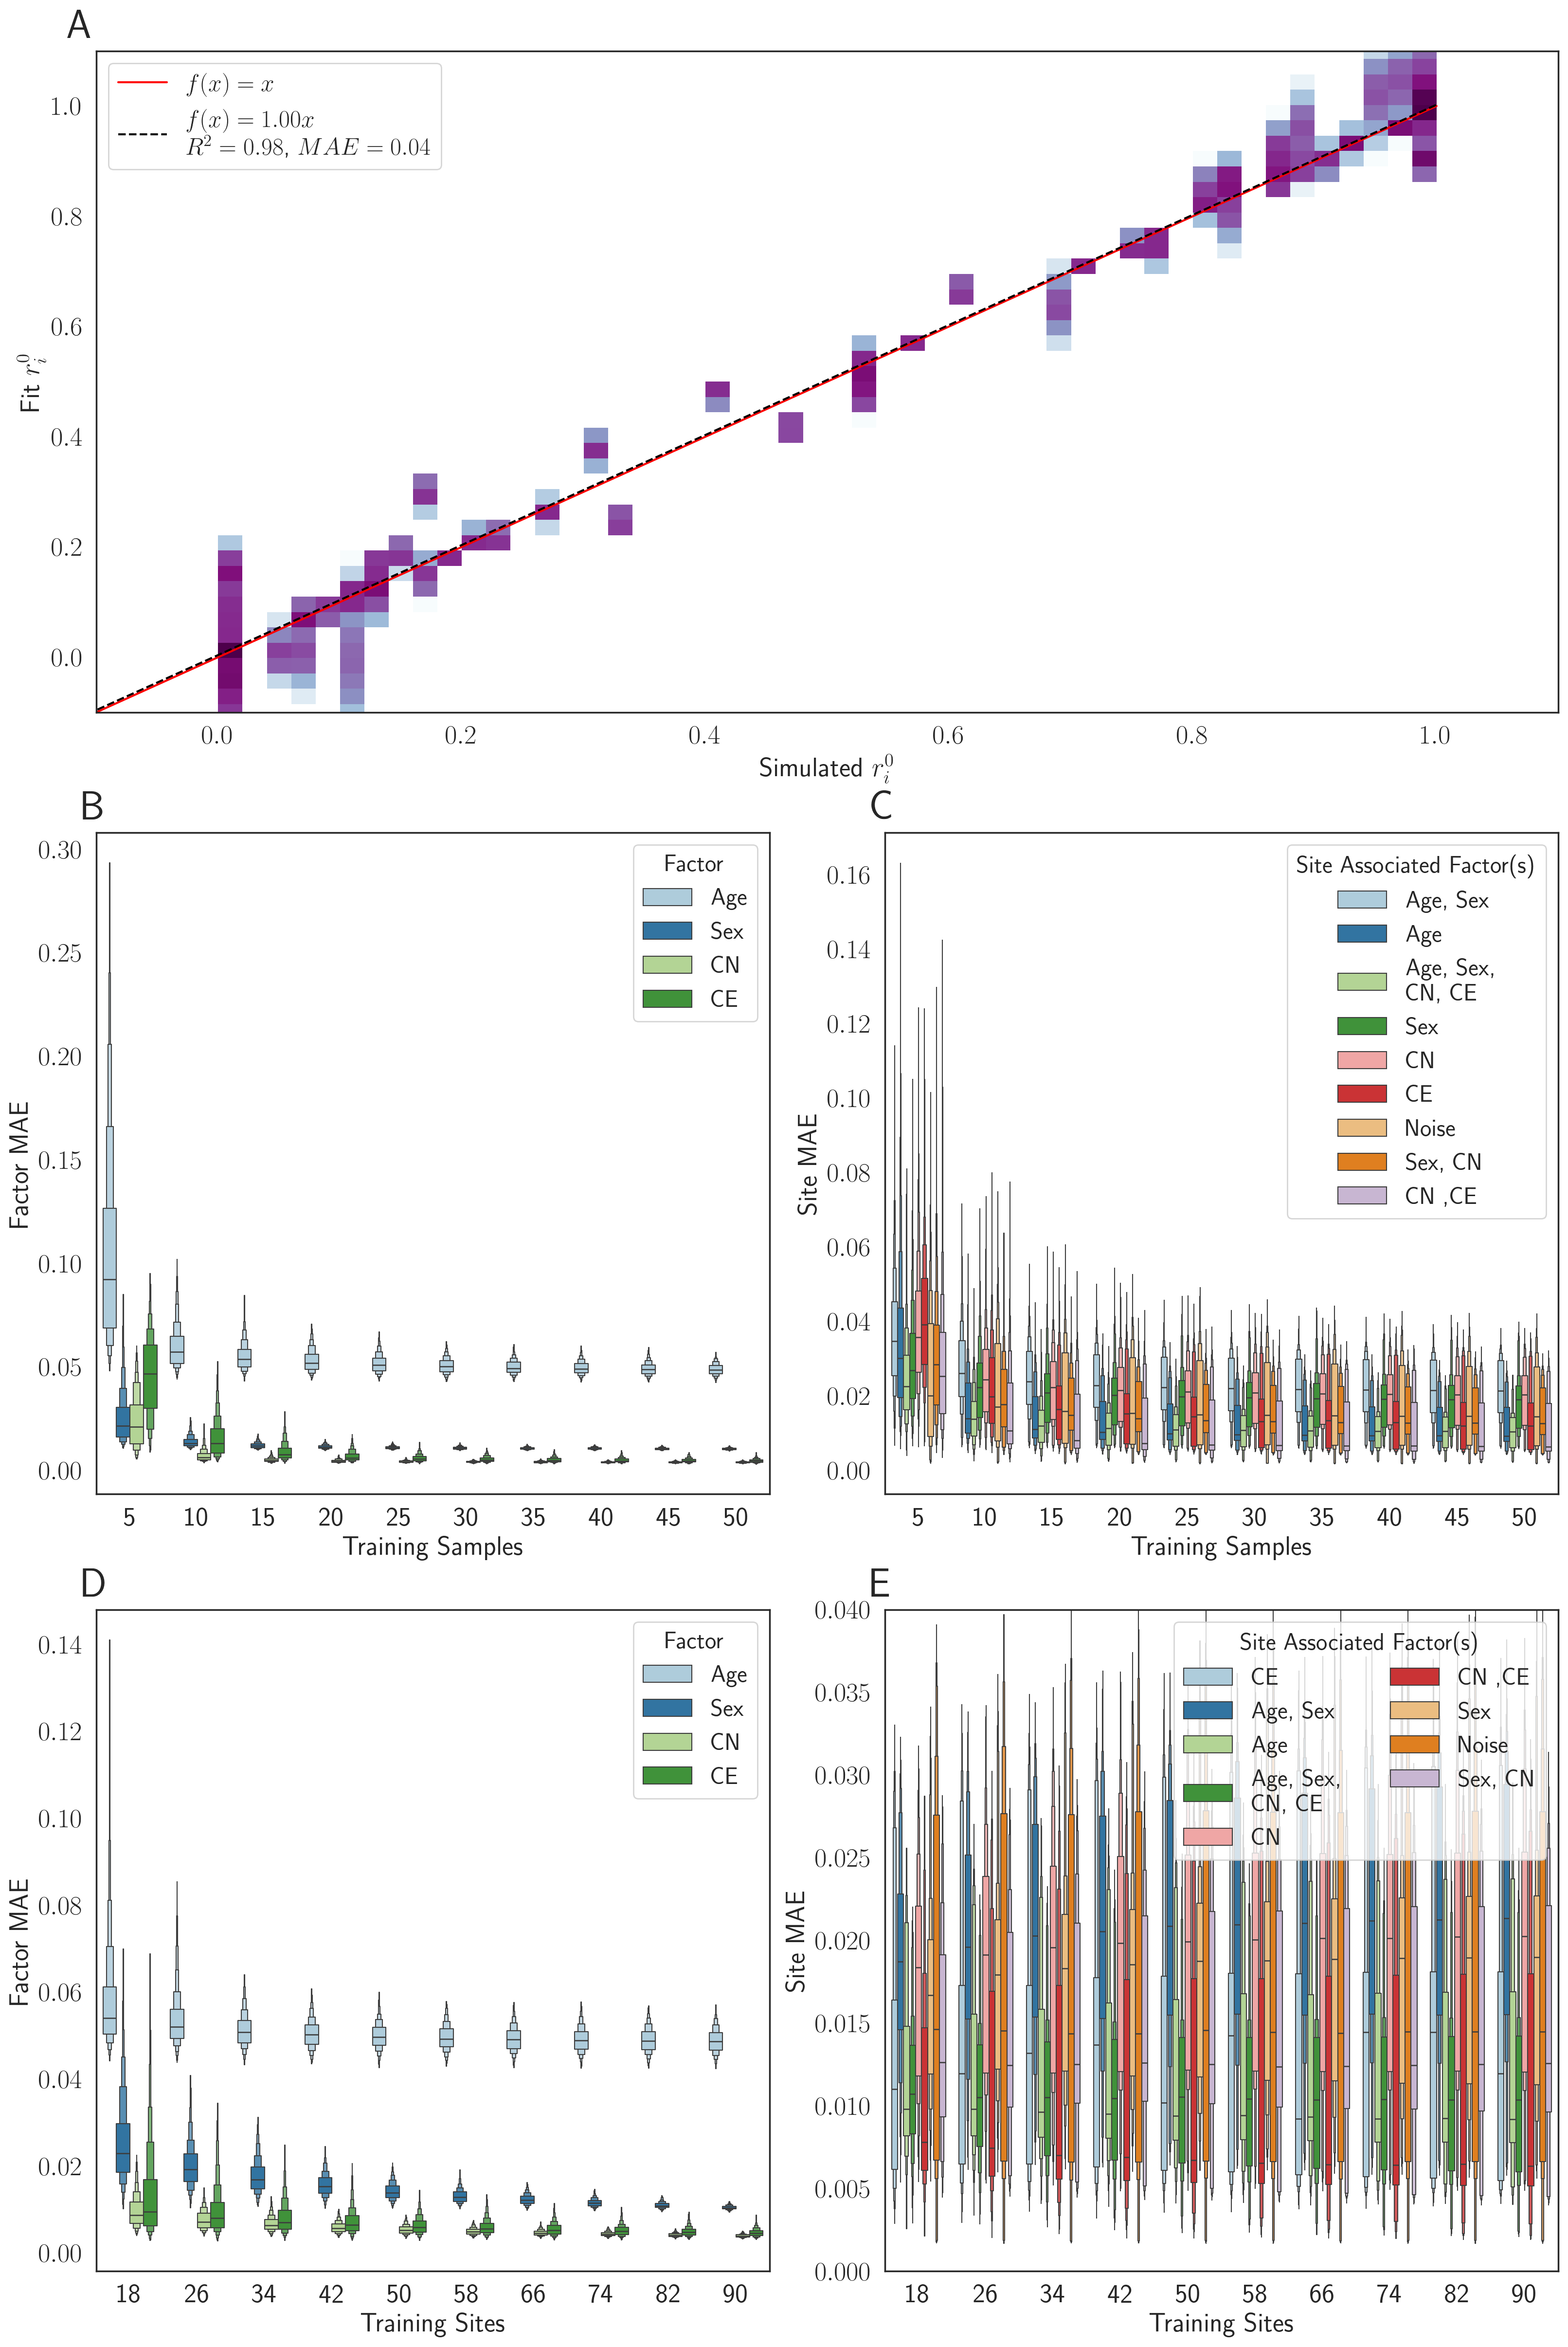
\includegraphics[scale=.2]{Figures/SupplementalFigure1.png}
    \footnotesize
    \caption*{\small \textbf{Supp. Figure 1: } Simulated methylation site intercept accurately modeled with 
    MSEPM four factor model (A).  Simulation phenotype  (B) and site methylation (C) prediction 
    MAE for four-factor MSEPM models fit with a varying number of training samples and sites (D-E).
 
    }
    \end{figure}
\end{center}

\begin{center}
    \begin{figure}
    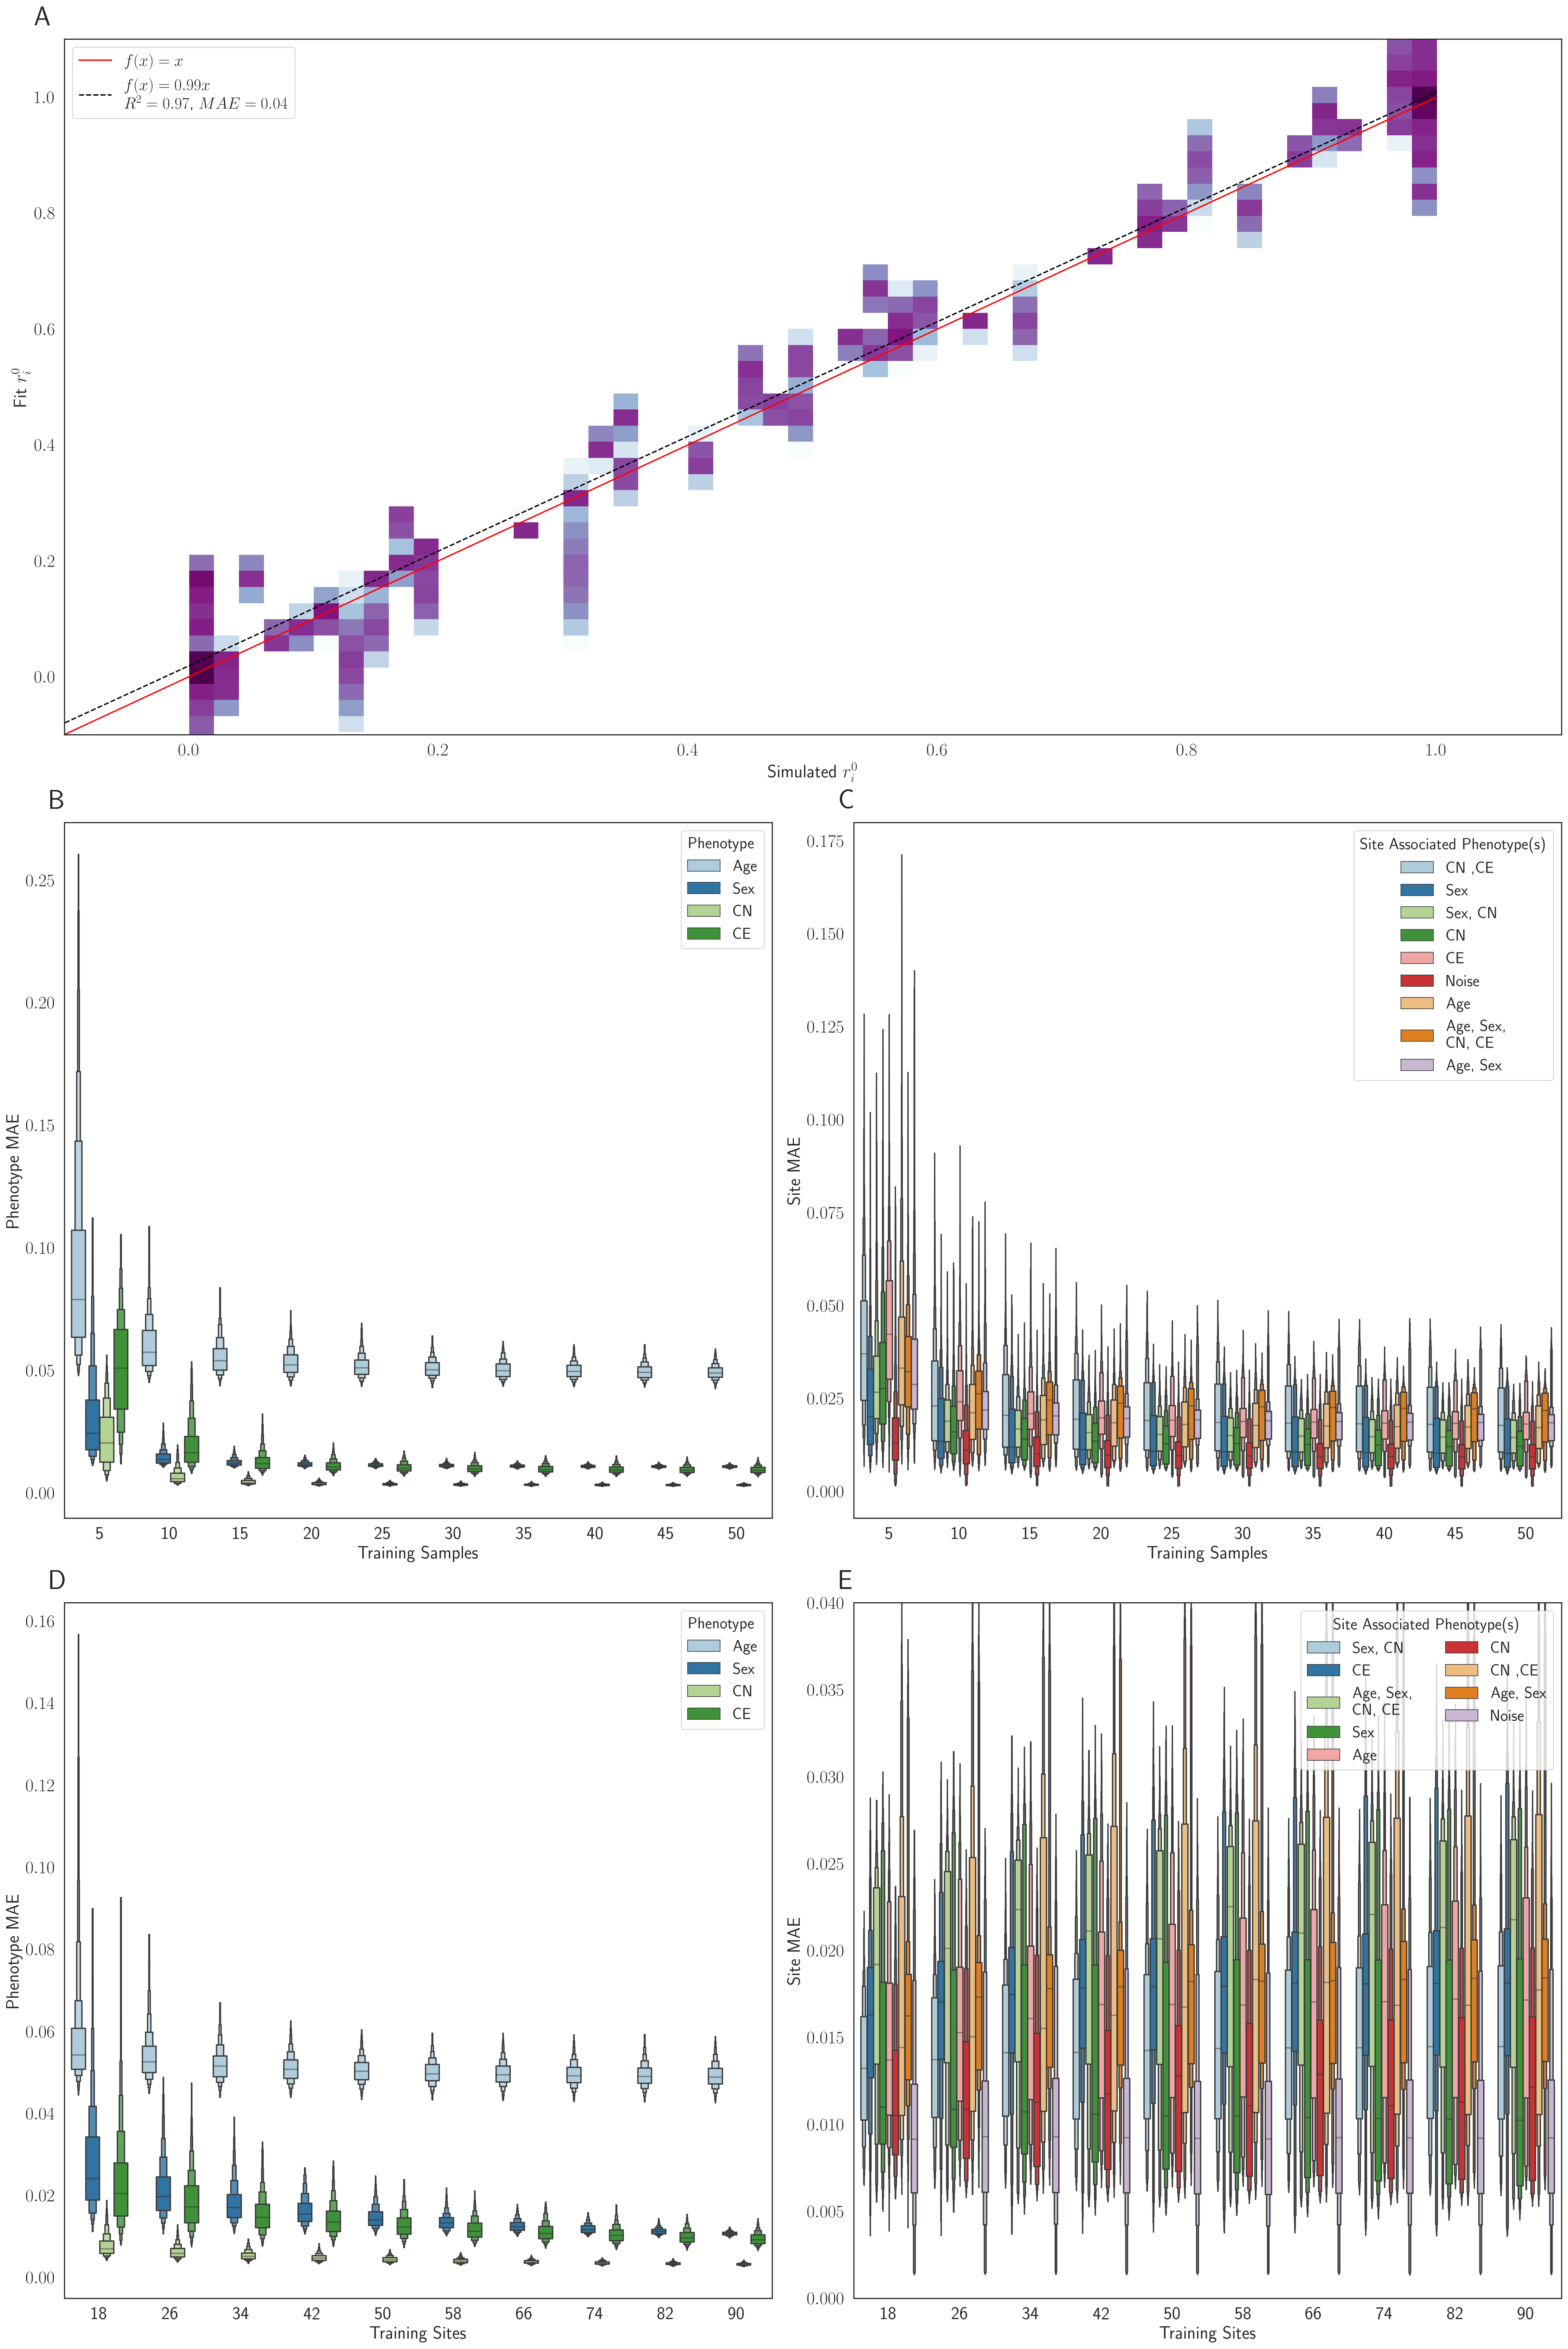
\includegraphics[scale=.1]{Figures/SupplementalFigure2.png}
    \footnotesize
    \caption*{\small \textbf{Supp. Figure 2: } MSEPM testing blood model predictions for MSEPM model fit 
    with only age (first row), age / sex (second row), age / sex / cell type PC1 (third row), and age / 
    sex / cell type PC1 / cell type PC2 (fourth row).
    }
    \end{figure}
\end{center}

\begin{center}
    \begin{figure}
    \includegraphics[scale=.1]{Figures/SupplementalFigure3.png}
    \footnotesize
    \caption*{\small \textbf{Supp. Figure 3: } Simulated testing model predictions for MSEPM model fit with only age 
    (first row), age / sex (second row), age / sex / CN (third row), and age / sex / 
    cell type PC1 / cell type PC2 (fourth row).
    }
    \end{figure}
\end{center}

\begin{center}
    \begin{figure}
    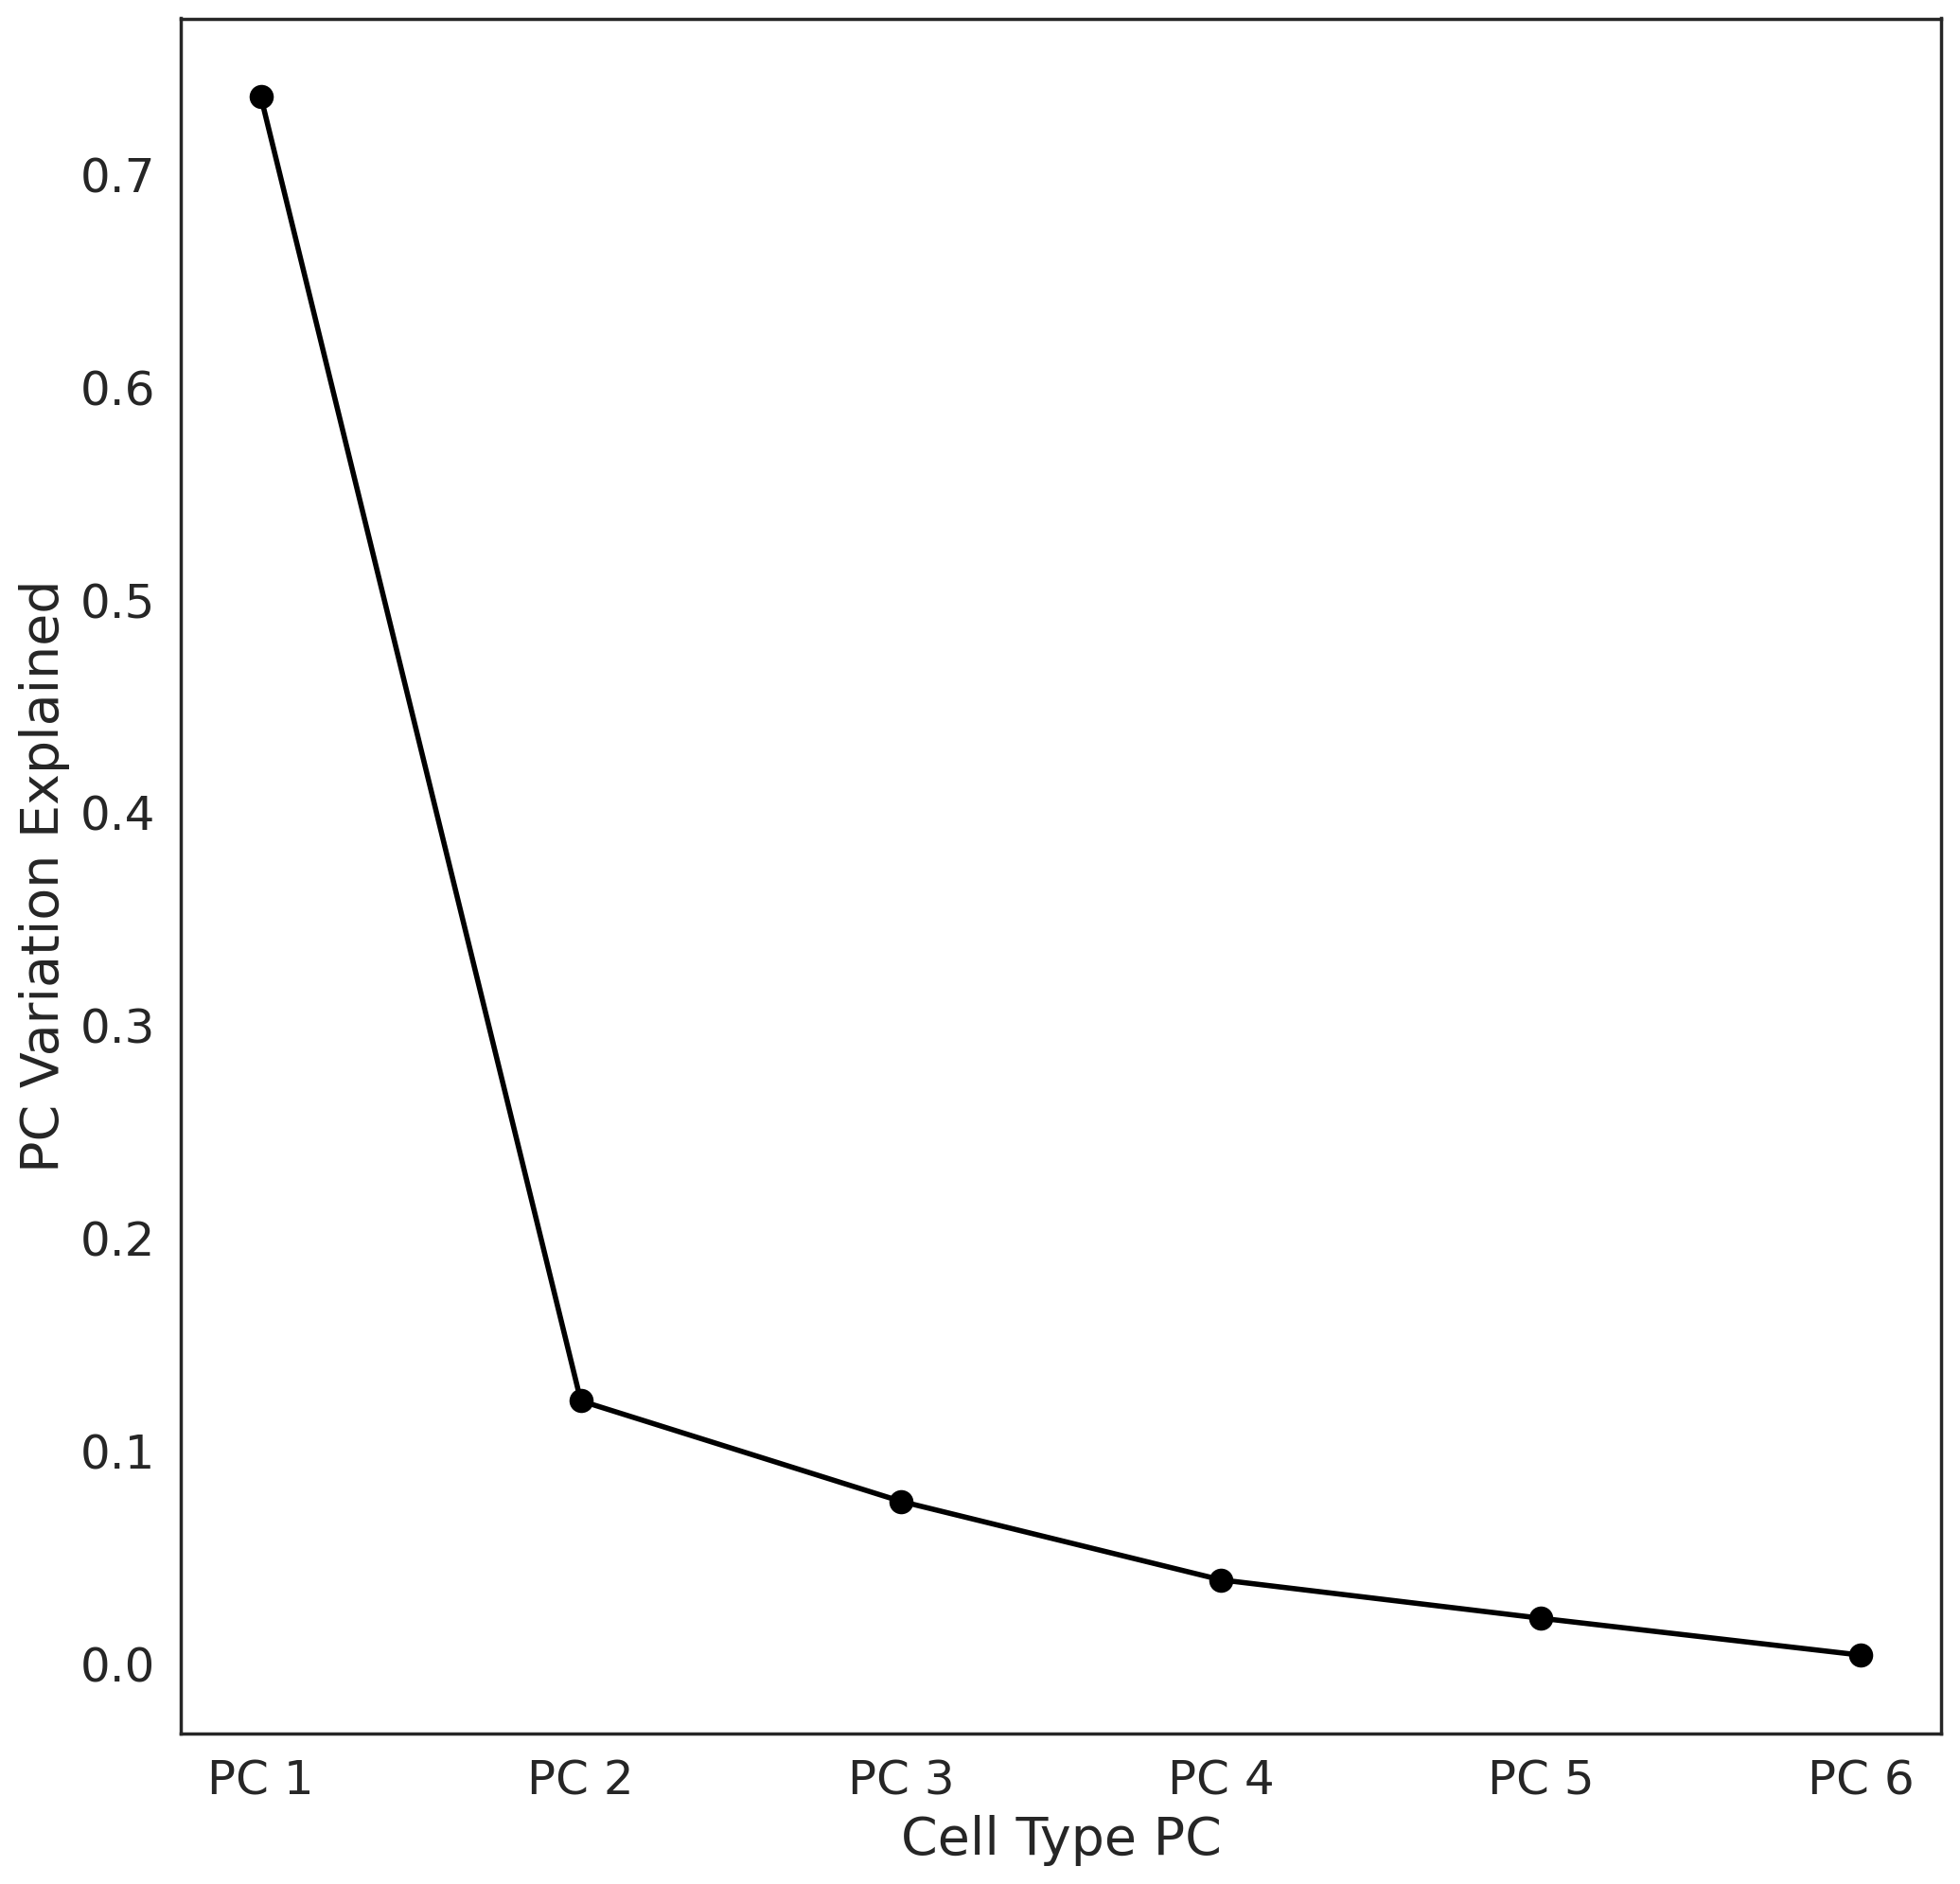
\includegraphics[scale=.4]{Figures/SupplementalFigure4.png}
    \footnotesize
    \caption*{\small \textbf{Supp. Figure 4: } Cell type principal component analysis scree plot.

    }
    \end{figure}
\end{center}

\begin{center}
    \begin{figure}
    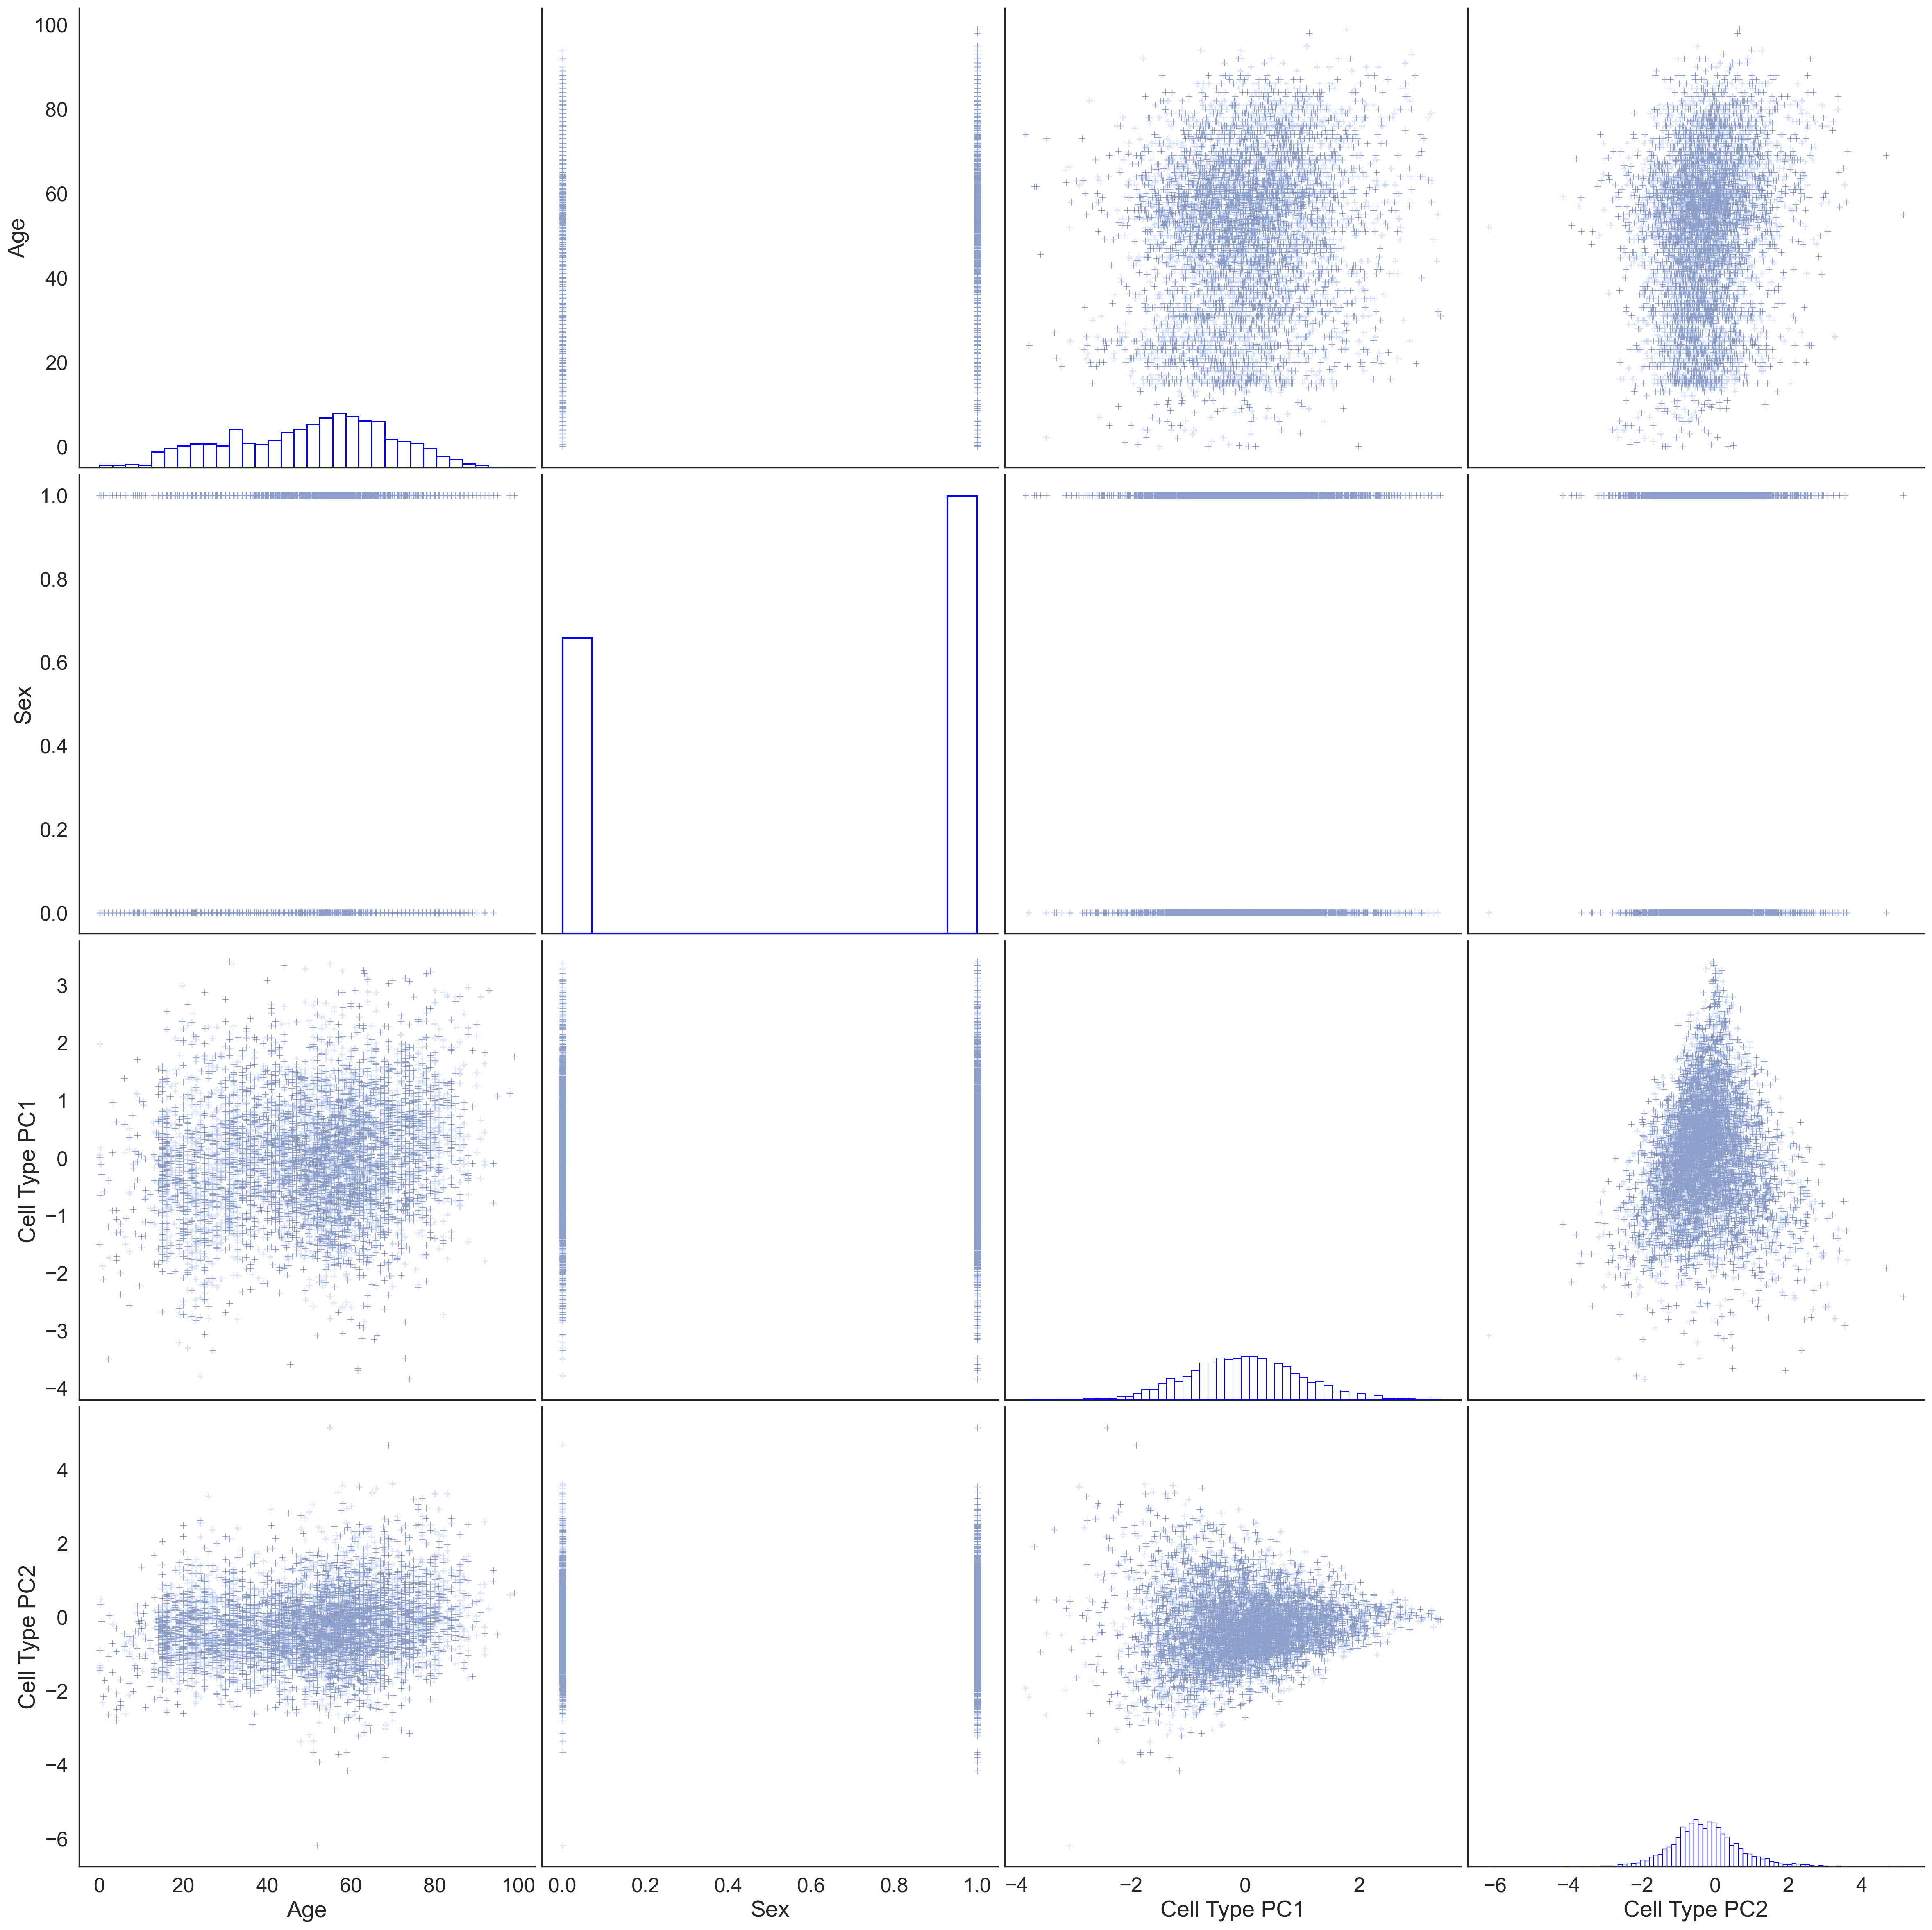
\includegraphics[scale=.2]{Figures/SupplementalFigure5.png}
    \footnotesize
    \caption*{\small \textbf{Supp. Figure 5: } Pairwise bivariate distributions, and single factor distributions 
    plots, for GEO factor data (age, sex, CT PC1 and CT PC2) used in MSEPM model training. 
    }
    \end{figure}
\end{center}

\begin{center}
    \begin{figure}
    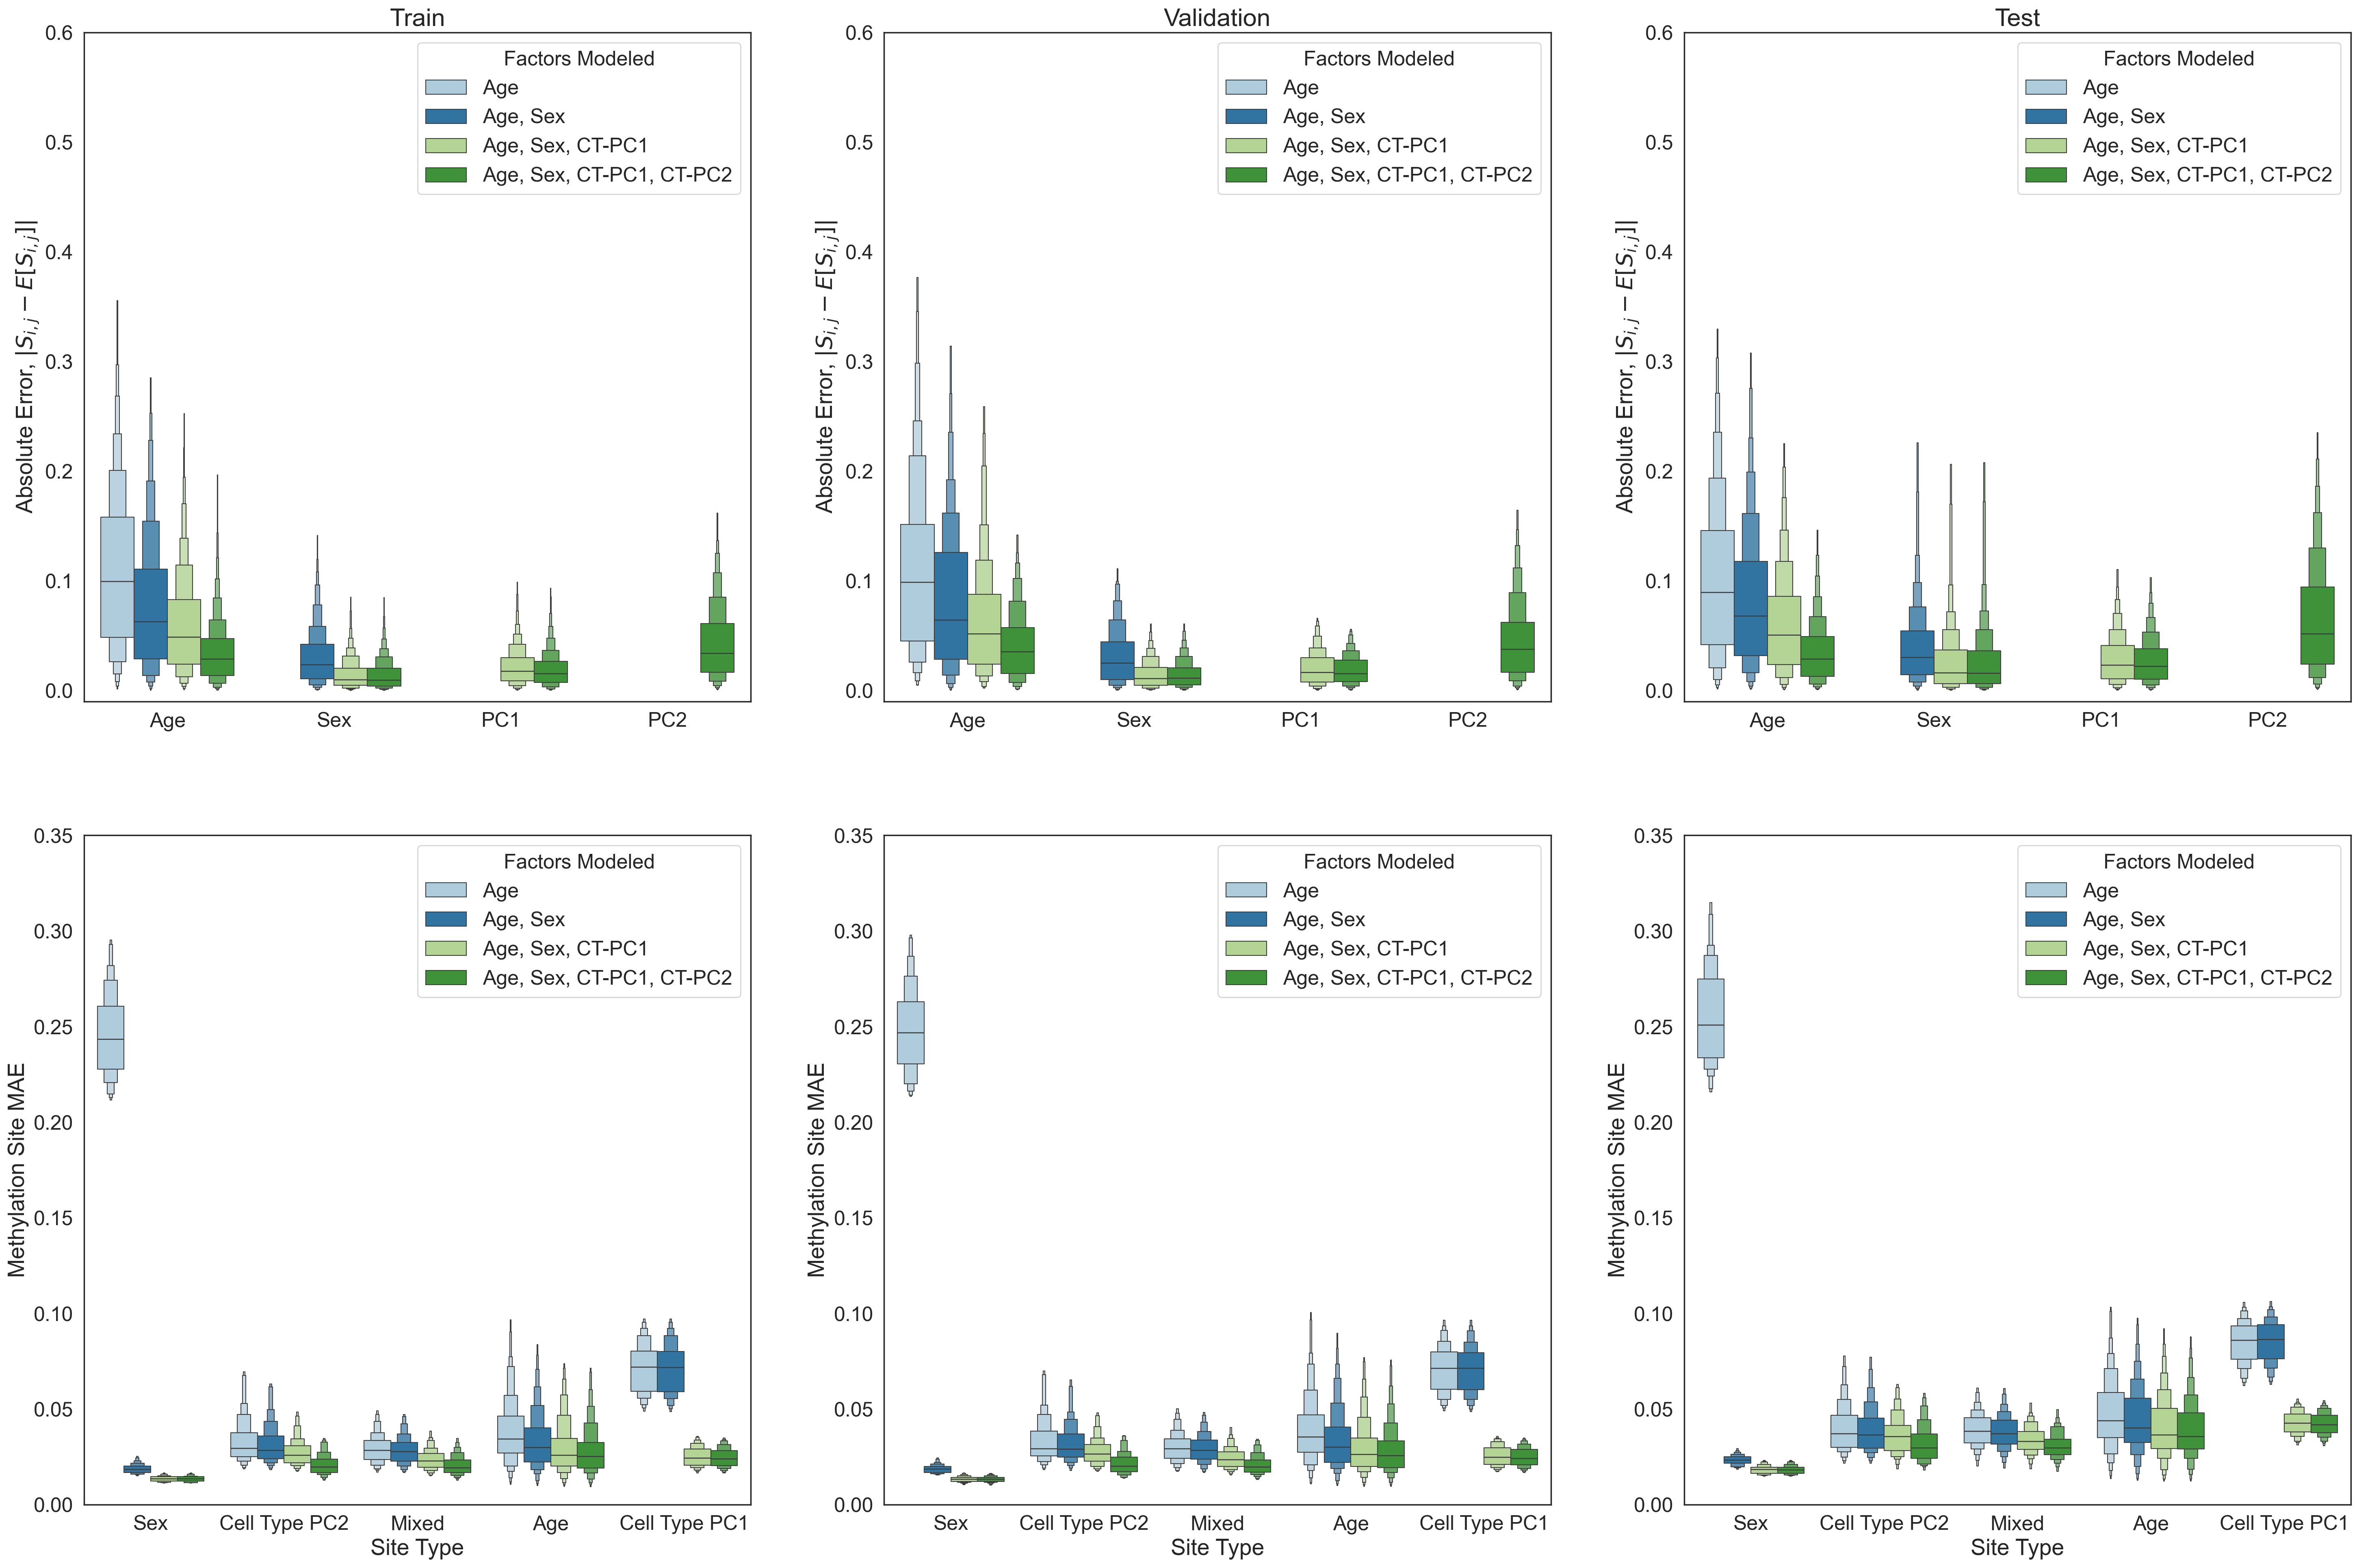
\includegraphics[scale=.18]{Figures/SupplementalFigure6.png}
    \footnotesize
    \caption*{\small \textbf{Supp. Figure 6: } Methylation site and sample factor prediction error for models 
    trained with 1 to 4 factors for training, validation and testing sets. 
    }
    \end{figure}
\end{center}

\begin{center}
    \begin{figure}
    \includegraphics[scale=.1]{Figures/SupplementalFigure7.png}
    \footnotesize
    \caption*{\small \textbf{Supp. Figure 7: } MSEPM blood model predictions for MSEPM model fit against age, sex, 
    CT PC1 and CT PC2 for training, validation and testing sets. 
    }
    \end{figure}
\end{center}

\end{document}